\documentclass[9pt,mathserif]{beamer}
\usepackage{etex}
%\documentclass[9pt,mathserif,handout]{beamer}
\mode<presentation>
{
  \usetheme{Warsaw}
  \usecolortheme{crane}
  \setbeamercovered{transparent}
	\useoutertheme{split} 
	 
	\defbeamertemplate*{slidenumber}{framenumber} 
	     {\insertframenumber} 
	 \defbeamertemplate{slidenumber}{totalframenumber} 
	     {\insertframenumber\,/\,\inserttotalframenumber} 
	 \defbeamertemplate{slidenumber}{pagenumber} 
	     {\insertpagenumber} 
	 \defbeamertemplate{slidenumber}{totalpagenumber} 
	     {\insertpagenumber\,/\,\insertpresentationendpage} 
	 
	\defbeamertemplate*{footline}{split slidenumber right} 
	 {% 
	   \leavevmode% 
	   \hbox{\begin{beamercolorbox}
	[wd=.5\paperwidth,ht=2.5ex,dp=1.125ex,leftskip=.3cm plus1fill,rightskip=.3cm]
	{author in head/foot}% 
	     \usebeamerfont{author in head/foot}\insertshortauthor 
	   \end{beamercolorbox}% 
	   \begin{beamercolorbox}
	[wd=.5\paperwidth,ht=2.5ex,dp=1.125ex,leftskip=.3cm,rightskip=.3cm plus1fil]
	{title in head/foot}% 
	     \usebeamerfont{title in head/foot}\insertshorttitle% 
	     \hskip2ex plus1fill% 
	     \usebeamertemplate{slidenumber}% 
	   \end{beamercolorbox}}% 
	   \vskip0pt% 
	 
	} 
	 
	\defbeamertemplate{footline}{split slidenumber left} 
	 {% 
	   \leavevmode% 
	   \hbox{\begin{beamercolorbox}
	[wd=.5\paperwidth,ht=2.5ex,dp=1.125ex,leftskip=.3cm plus1fil,rightskip=.3cm]
	{author in head/foot}% 
	     \usebeamerfont{author in head/foot}% 
	     \usebeamertemplate{slidenumber}% 
	     \hskip2ex plus1fill% 
	     \insertshortauthor 
	   \end{beamercolorbox}% 
	   \begin{beamercolorbox}
	[wd=.5\paperwidth,ht=2.5ex,dp=1.125ex,leftskip=.3cm,rightskip=.3cm plus1fil]
	{title in head/foot}% 
	     \usebeamerfont{title in head/foot}\insertshorttitle% 
	   \end{beamercolorbox}}% 
	   \vskip0pt% 
	} 
}


\usepackage[english]{babel}
\usepackage[latin1]{inputenc}
\usepackage{times}
\usepackage[T1]{fontenc}
\usepackage{verbatim}

\usepackage{amsmath}
\usepackage{amssymb}
\usepackage{amsfonts}
\usepackage{pxfonts}
\usepackage{amsthm}
\usepackage{graphicx}
\usepackage{stmaryrd}


\usepackage{bussproofs}
\usepackage{proof}

\usepackage{fancybox}
\usepackage{fancyvrb}


% \usepackage{tikz}
% \usepackage{pgfgantt}
% \usepackage{chronology}


%\usepackage{rotating}

% Sequent Calculus Proof Settings
\EnableBpAbbreviations
\def\fCenter{\mbox{\ $\vdash$\ }}

\usepackage{calculi}

\newcommand\hol[1]{\boldsymbol{#1}}
\newcommand\lift[1]{\lceil #1 \rceil}
\newcommand\llift[1]{\dot{#1}}

\newcommand{\imp}{\supset}
\newcommand{\biimp}{\equiv}
\newcommand{\allq}{\forall}
\newcommand{\all}{\forall}
\newcommand{\exq}{\exists}
\newcommand{\ex}{\exists}
\newcommand{\seq}{\vdash}
\newcommand{\nec}{\Box} % necessarily
\newcommand{\pos}{\Diamond} % possibly
\newcommand{\ess}[2]{#1 \ \mathit{ess.} \ #2}
\newcommand{\NE}{\mathit{NE}}

\newcommand{\s}{\qquad}

\def\modal#1{\boldsymbol{#1}}
\def\mfalse{\modal\bot}
\def\mtrue{\modal\top}
\def\mnot{\modal\neg\,}
\def\mor{\,\modal\vee\,}
\def\mand{\,\modal\wedge\,}
\def\mimpl{\,\modal\supset\,}
\def\miff{\,\modal\Leftrightarrow\,}
\def\mball#1{\modal\Box_{#1}\,}
\def\mdexi#1{\modal\Diamond_{#1}\,}
\def\mall#1{\modal{\forall}{#1}\lambdot\,}
\def\mallprop#1{\modal{\forall^{p}}{#1}\lambdot\,}
\def\mallind#1{\modal{\forall^{\mu}}{#1}\lambdot\,}
\def\mexi#1{\modal{\exists}{#1}\lambdot\,}
\def\mpi{\modal{\Pi}\,}
\def\mvalid{\modal{\texttt{valid}}} 

\def\typearrow{\shortrightarrow}
\def\worldtype{\iota}
\def\indtype{\mu}


\newenvironment{transitionframe}[2]
{
\begin{frame}{} \Large
\centering
\colorbox{#2}{\includegraphics[height=.6\textheight]{#1}}
\vfill
}
{

\end{frame}
}

\newenvironment{changemargin}[2]{% 
  \begin{list}{}{% 
    \setlength{\topsep}{0pt}% 
    \setlength{\leftmargin}{#1}% 
    \setlength{\rightmargin}{#2}% 
    \setlength{\listparindent}{\parindent}% 
    \setlength{\itemindent}{\parindent}% 
    \setlength{\parsep}{\parskip}% 
  }% 
\item[]
}{\end{list}} 


\def\scottproof{
\resizebox{\textwidth}{!}{
\begin{minipage}{12cm}%\small
\begin{itemize}
\item[Axiom A1] Either a property or its negation is positive, but not
  both: \hfill 
  ${\allq \phi [P(\neg \phi) \biimp \neg P(\phi)]}$ 
\item[Axiom A2] A property necessarily implied by a
  positive property is positive:  \phantom{bla bla bla bla bla bla bla}  \hfill 
  ${\allq \phi \allq \psi [(P(\phi) \wedge \nec \allq x [\phi(x)
  \imp \psi(x)]) \imp P(\psi)]}$ 
\item[\textcolor{blue}{Thm. T1}] \textcolor{blue}{Positive properties are possibly exemplified:} \hfill \textcolor{blue}{${\allq
  \phi [P(\phi) \imp \pos \exq x \phi(x)]}$}
\item[Def. D1] A \emph{God-like} being possesses all positive properties: \hfill
  ${G(x) \biimp \forall \phi [P(\phi) \imp \phi(x)]}$ 
\item[Axiom A3]  The property of being God-like is positive: \hfill   ${P(G)}$ 
\item[\textcolor{blue}{Cor. C\phantom{1}}] \textcolor{blue}{Possibly, God exists:}\hfill \textcolor{blue}{${\pos \exq x G(x)}$}
\item[Axiom A4]  Positive properties are necessarily positive: \hfill 
  ${\allq \phi [P(\phi) \imp \Box \; P(\phi)]}$ 
\item[Def. D2] An \emph{essence} of an individual is a property possessed by it and necessarily implying any of its properties: \hfill ${\ess{\phi}{x} \biimp \textcolor{red}{\phi(x)\,\wedge\,}\allq
  \psi (\psi(x) \imp \nec \allq y (\phi(y) \imp \psi(y)))}$ 
\item[\textcolor{blue}{Thm. T2}]  \textcolor{blue}{Being God-like is an essence of any
  God-like being:}  \hfill \textcolor{blue}{${\allq x [G(x) \imp \ess{G}{x}]}$}
\item[Def. D3] \emph{Necessary existence} of an individ.~is the necessary exemplification of all its essences: 
  \phantom{b} \hfill ${\NE(x) \biimp \allq \phi [\ess{\phi}{x} \imp \nec
  \exq y \phi(y)]}$
\item[Axiom A5] Necessary existence is a positive property: \hfill ${P(\NE)}$ 
\item[\textcolor{blue}{Thm. T3}] \textcolor{blue}{Necessarily, God exists:} \hfill \textcolor{blue}{${\nec \exq x G(x)}$}
\end{itemize}
\end{minipage}
}}

\title{G�del's Proof of God's Existence}
\author{\textbf{Christoph Benzm\"{u}ller} and \textbf{Bruno Woltzenlogel Paleo}}

% \institute[]{
%   \inst{}%
% }


\date{Square of Opposition \\
Vatican, May 6, 2014}

\begin{document}




\begin{frame}
  \titlepage
\colorbox{gray}{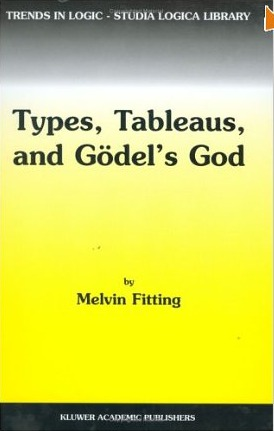
\includegraphics[height=2.5cm]{$HOME/GoedelGod/Talks/FU-Berlin/Images/Books/buch7.jpg} }
\hfill
\colorbox{gray}{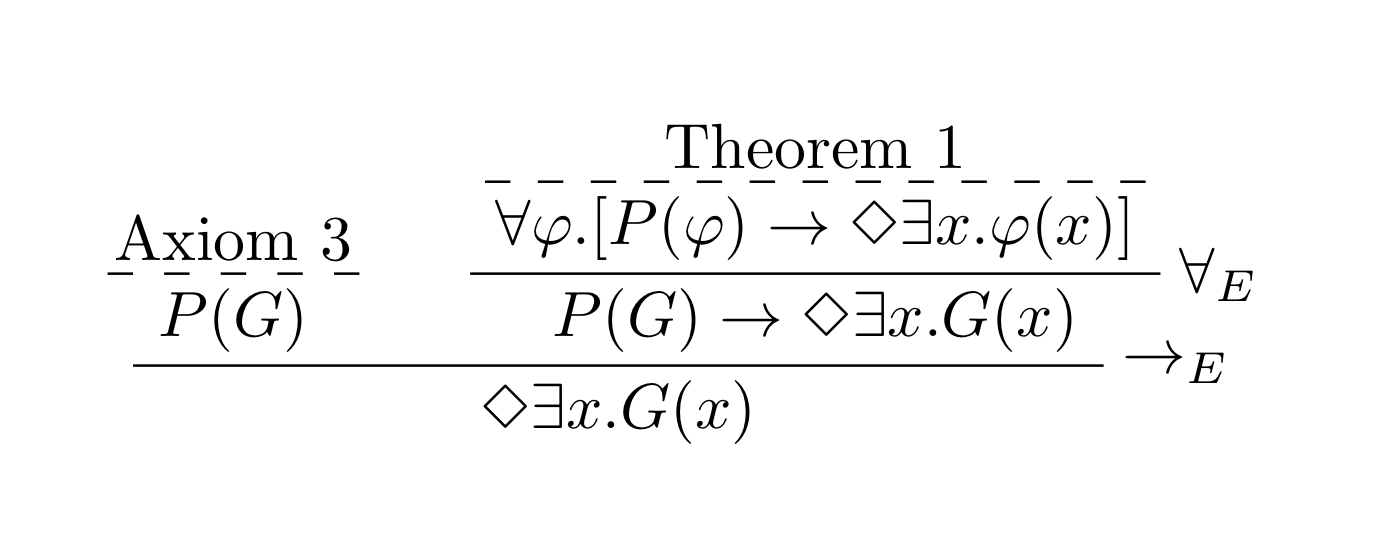
\includegraphics[height=2cm]{$HOME/GoedelGod/Talks/FU-Berlin/Images/ND.png}}

\hfill \begin{footnotesize}A gift to \textbf{Priest Edvaldo} in Piracicaba, Brazil\end{footnotesize}
\end{frame}

\author{\textbf{Christoph Benzm\"{u}ller} and \textbf{Bruno
    Woltzenlogel Paleo}}



\begin{frame}{Contribution}\Large
\colorbox{gray}{
\begin{minipage}{.9\textwidth} 
\textcolor{white}{First time mechanization and automation of}
\begin{itemize}
\item \textcolor{white}{(variants of) a  modern ontological argument}
\item \textcolor{white}{(variants of) higher-order modal logic}
\end{itemize}
\end{minipage}
}
\vfill
Work context/history:
\begin{itemize}
\item Proposal: HOL as a (quite) universal logic via elegant
  semantic embeddings --- cf. previous
  talk at UNILOG
  \begin{itemize}
  \item for object-level reasoning
  \item for meta-level reasoning
  \end{itemize}
\item Proof of concept: Demonstrate practical relevance of the approach by
  an interesting and relevant application
\item Experiments: Systematic study of G�del's argument
% \item Results: Verification  of known results / partly novel results
\item Relation to Square of Opposition: should be easy to analyze variants of
  the Square within our approach
\end{itemize}
\end{frame}



\begin{frame}{Introduction} \large
\hskip-1em Challenge: \hfill No provers for \emph{Higher-order Quantified Modal Logic\/} (\textcolor{red}{QML}) \\[1em]

\hskip-1em Our solution: \hfill Embedding in \emph{Higher-order Classical Logic\/} (\textcolor{blue}{HOL}) \\
%\,\hfill {\small [Benzm\"ullerPaulson, Logica Universalis, 2013]} \\[2em]

\hskip-1em What we did: \\

\begin{itemize}
\item[A:] Pen and paper: \hfill detailed natural deduction proof 
\item[B:] Formalization: \hfill in classical higher-order logic (\textcolor{blue}{HOL})
\item[] Automation: \hfill theorem provers \textsc{LEO-II(\textbf{E})} and \textsc{Satallax} 
\item[] Consistency: \hfill model finder \textsc{Nitpick (Nitrox)} 
\item[C:] Step-by-step verification: \hfill proof assistant \textsc{Coq} 
\item[D:] Automation \& verification: \hfill proof assistant \textsc{Isabelle} \\[2em]
%\item[ ] Conclusion \\[2em]
\end{itemize}
\hskip-1em  Did we get any new results? \hfill  \textcolor{red}{We
  think: Yes --- let's discuss this later!}
\end{frame}

% \begin{transitionframe}{Images/Transitions/RioChrist3}{black}
% \textbf{Part A:}

% Informal Proof and Natural Deduction Proof
% \end{transitionframe}



\begin{frame}{Introduction} \small
\vskip1em
\begin{minipage}{.56\textwidth} 
\onslide*<1-2>{
\onslide*<1>{\colorbox{gray}{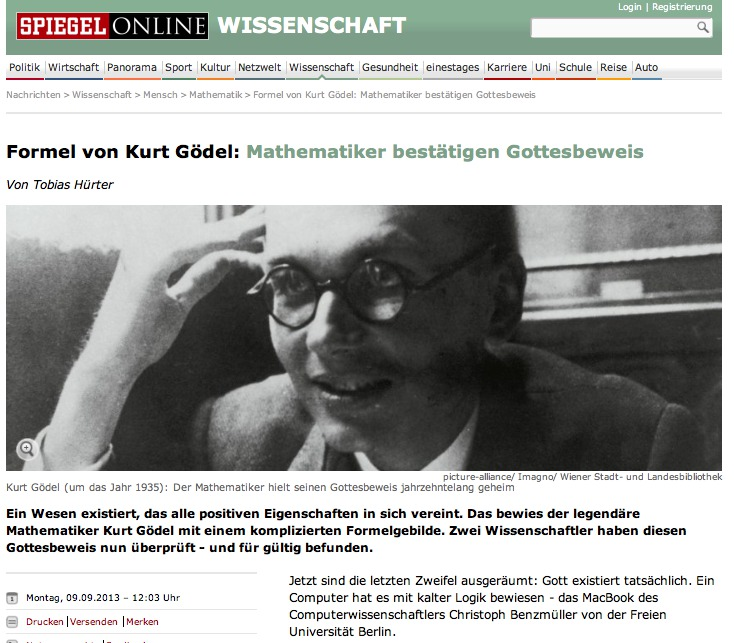
\includegraphics[width=.95\textwidth]{$HOME/GoedelGod/Talks/FU-Berlin/Images/News/spiegel1}}}
\onslide*<2>{\colorbox{gray}{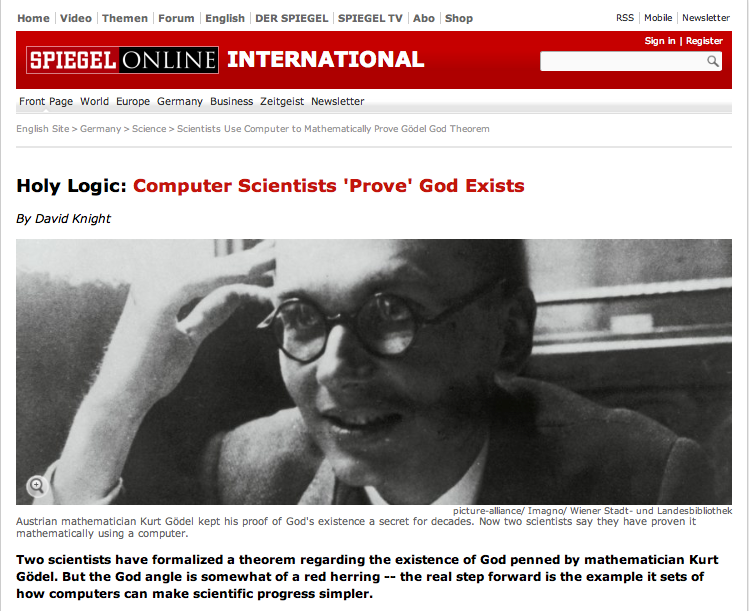
\includegraphics[width=\textwidth]{$HOME/GoedelGod/Talks/FU-Berlin/Images/News/spiegel2}}}
\vskip1em
Germany \\
- Telepolis \& Heise \\
- Spiegel Online \\
- FAZ \\
- Die Welt \\
- Berliner Morgenpost \\
- Hamburger Abendpost \\
- \ldots \\
}
%\onslide*<3>{\colorbox{gray}{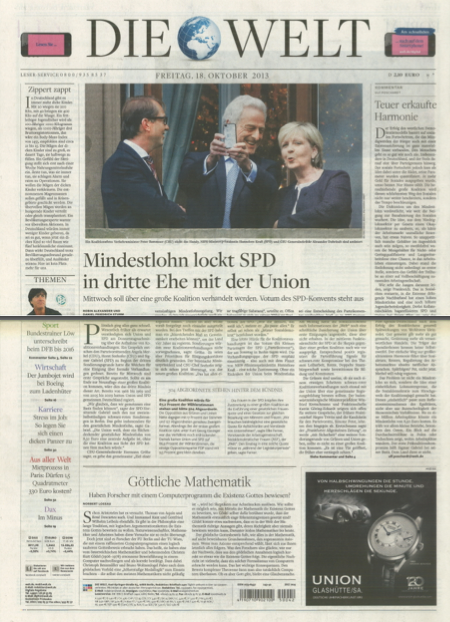
\includegraphics[width=\textwidth]{$HOME/GoedelGod/Talks/FU-Berlin/Images/News/welt}}}
\end{minipage} \hfill
%
\begin{minipage}{.3\textwidth}
Austria \\
- Die Presse \\
- Wiener Zeitung \\
- ORF \\
- \ldots \\

Italy \\
- Repubblica \\
- Ilsussidario \\
- \ldots \\

% Russia \\
% - \ldots \\

India \\
- DNA India \\
- Delhi Daily News \\
- India Today \\
- \ldots \\

US \\
- ABC News \\
- \ldots \\

International \\
- Spiegel International \\
- Yahoo Finance \\
% - CNET \\
- United Press Intl. \\
- \ldots \\
\end{minipage}
\end{frame}

\begin{frame}{Introduction} \large
\colorbox{gray}{
\includegraphics[width=\textwidth]{$HOME/GoedelGod/Talks/FU-Berlin/Images/News/MacBookGrab}} 
\pause
\vfill
% Are we in contact with Steve Jobs? \hfill No \\[2em]
Do you really need a MacBook to obtain the results? \hfill No \\[2em]
Did Apple send us some money? \hfill No \\
%\, \hfill (but maybe they should)
\end{frame}



\begin{frame}{Introduction} \Large
{Rich history on ontological arguments (\textcolor{blue}{pros} and \textcolor{red}{cons})}\\[1em]

\hskip-.5em
\ldots\rotatebox[origin = bl,width = 0mm]{65}{\textcolor{blue}{Anselm v. C.}} \hskip-2.3em
          \rotatebox[origin = bl]{65}{\textcolor{red}{Gaunilo}} \hskip-1.3em
\ldots  \rotatebox[origin = bl]{65}{\textcolor{red}{Th. Aquinas}}  \hskip-2.3em
\ldots\ldots   \rotatebox[origin = bl]{65}{\textcolor{blue}{Descartes}} \hskip-1.7em
               \rotatebox[origin = bl]{65}{\textcolor{blue}{Spinoza}} \hskip-1.3em
               \rotatebox[origin = bl]{65}{\textcolor{blue}{Leibniz}}  \hskip-1.2em
\ldots  \rotatebox[origin = bl]{65}{\textcolor{red}{Hume}}  \hskip-1em
          \rotatebox[origin = bl]{65}{\textcolor{red}{Kant}}  \hskip-.8em
\ldots  \rotatebox[origin = bl]{65}{\textcolor{blue}{Hegel}}  \hskip-1.3em
\ldots  \rotatebox[origin = bl]{65}{\textcolor{red}{Frege}}  \hskip-1.3em
\ldots  \rotatebox[origin = bl]{65}{\textcolor{blue}{Hartshorne}} \hskip-1.9em
          \rotatebox[origin = bl]{65}{\textcolor{blue}{Malcolm}}  \hskip-1.4em
          \rotatebox[origin = bl]{65}{\textcolor{red}{Lewis}}  \hskip-1em
          \rotatebox[origin = bl]{65}{\textcolor{blue}{Plantinga}}  \hskip-1.6em
          \rotatebox[origin = bl]{65}{\textcolor{blue}{G\"odel}}   \hskip-1.2em
\ldots \\[1em]

\pause
\vfill
Anselm's notion of God:\\
\,\hfill \emph{``God is that, than which nothing greater can be
  conceived.''} \\[1em]

G\"odel's notion of God:\\
\,\hfill \emph{``A God-like being possesses all `positive' properties.''} \\[1em]

To show by logical reasoning: \\
\,\hfill \emph{``(Necessarily) God exists.''} \\[1em]

% \rnode{n2}{}\emph{}
% \ncline[nodesep=2pt,linecolor=black,linewidth=1pt]{->}{n1}{n2}
\end{frame}


\begin{frame}{Introdcution} \Large
Different Interests in Ontological Arguments: \\[1em]
\begin{itemize}
\item \textcolor{blue}{Philosophical:} Boundaries of Metaphysics \& Epistemology
  \begin{itemize}
  \item We talk about a metaphysical concept (God), 
  \item but we want to draw
      a conclusion for the real world. % \\[1em]
 % \item Necessary Existence: metaphysical NE vs. logical NE  vs. modal NE 
   \\[2em]
  \end{itemize} 
\item \textcolor{blue}{Theistic:} Successful argument should convince atheists \\[2em]
\item \textcolor{red}{Ours:} Can computers (theorem provers) be used \ldots
  \begin{itemize}
  \item \ldots to formalize the definitions, axioms and theorems?
  \item \ldots to verify the arguments step-by-step?
  \item \ldots to fully automate (sub-)arguments? \\[2em]
  \end{itemize}
  Towards: \textcolor{red}{\emph{`Computer-assisted Theoretical
      Philosophy''}} \\[.5cm]
  (see e.g. the Computational Metaphysics Project of Ed Zalta and
  colleagues at Stanford University)
\end{itemize}
\end{frame}



\begin{frame}{G\"odel's Manuscript: 1930's, 1941, 1946-1955, 1970}
\bigskip

\begin{changemargin}{-1.2cm}{-1.2cm}
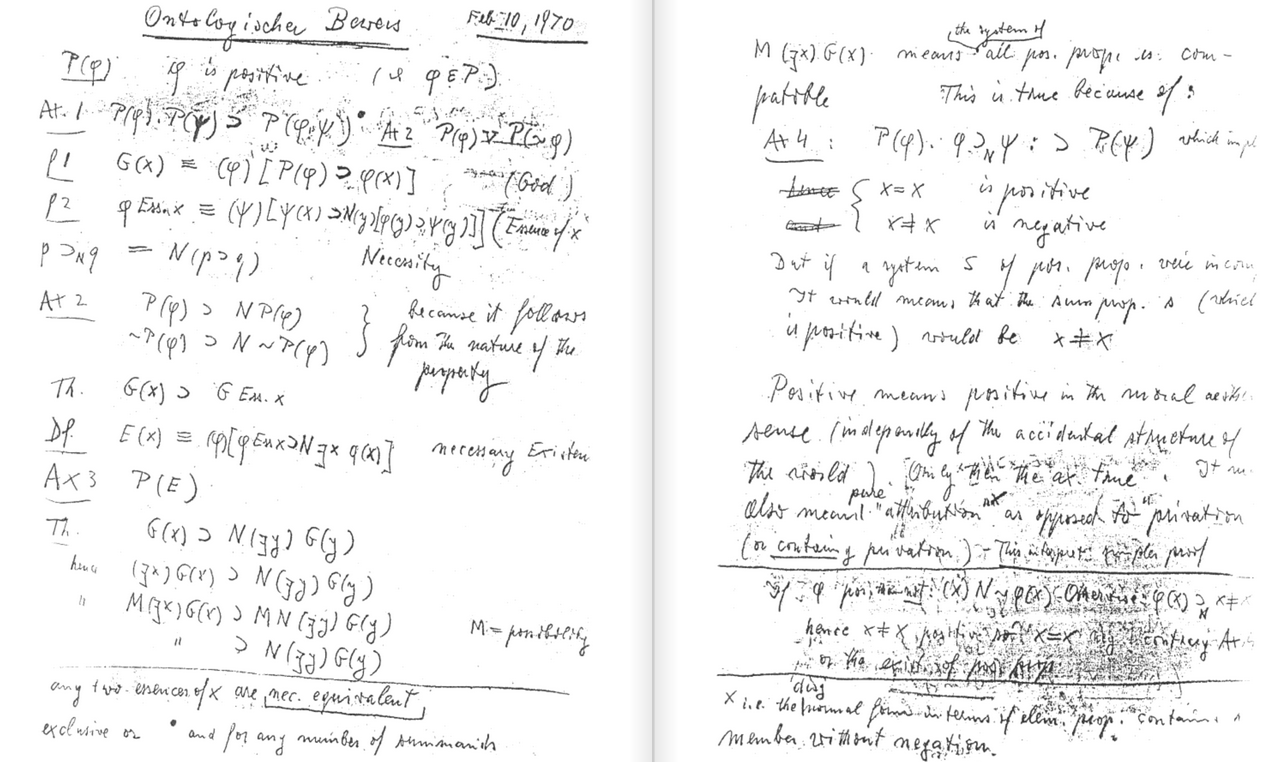
\includegraphics[width=13cm]{$HOME/GoedelGod/Talks/FU-Berlin/Images/Manuscript.png}
\end{changemargin}
\end{frame}

\begin{frame}{Scott's Version of G\"odel's Axioms, Definitions and
    Theorems}
\scottproof
\end{frame}


\begin{frame}{Remainder of this Talk}\Large
\begin{itemize}
\item Embedding of \textcolor{red}{QML} in \textcolor{blue}{HOL} and Proof Automation (myself)
\item Experiments and Results (Bruno)
\item Conclusion and Outlook (Bruno)
\end{itemize}
\end{frame}



\begin{transitionframe}{$HOME/GoedelGod/Talks/FU-Berlin/Images/Transitions/GodComputerC}{black}
\textbf{Embedding of \textcolor{red}{QML} in \textcolor{blue}{HOL}  and Proof Automation} \\[.5em]
% \quad Formalization: \hfill in classical higher-order logic (\textcolor{black}{HOL}) \\
% \quad Automation: \hfill theorem provers \textsc{Leo-II} and \textsc{Satallax} \\ 
% \quad Consistency: \hfill model finder \textsc{Nitpick (Nitrox)} \\
\end{transitionframe}

\begin{frame}{Formalization in HOL} \large

\hskip-1em Challenge: \hfill No provers for \emph{Higher-order
  Quantified Modal
  Logic\/} (\textcolor{red}{QML}) \\[1em]

\hskip-1em Our solution: \hfill Embedding in \emph{Higher-order Classical
  Logic\/} (\textcolor{blue}{HOL}) \\
\, \hfill Then use existing \textcolor{blue}{HOL} theorem provers for reasoning in \textcolor{red}{QML} \\
\,\hfill {\small [Benzm\"ullerPaulson, Logica Universalis, 2013]}
\\[2em]

\hskip-1em Previous empiricial findings:  \\[.5em]
\,\hfill Embedding of  \emph{First-order Modal Logic} in HOL works well 

\,\hfill {\small [Benzm\"ullerOttenRaths, ECAI, 2012]} \\
\,\hfill {\small [Benzm\"ullerRaths, LPAR, 2013]}
\end{frame}



\begin{frame}{Formalization in HOL} \large

\hskip-1em\textcolor{red}{QML} \hfill
$\begin{array}{lll}\textcolor{red}{\varphi,\psi} & ::= &
  \textcolor{red}{\ldots}  \mid \textcolor{red}{\neg
    \varphi} \mid \textcolor{red}{\varphi \wedge \psi} \mid
  \textcolor{red}{\varphi \imp \psi}  \mid \textcolor{red}{\Box
    \varphi} \mid \textcolor{red}{\Diamond \varphi}  \mid
  \textcolor{red}{\forall {x}\, \varphi} \mid
  \textcolor{red}{\exists {x}\, \varphi} 
\mid \textcolor{red}{\forall {P}\, \varphi} \end{array}$ \\[1em]


\begin{itemize}
\item Kripke style semantics (possible world semantics)\\[2em]
\end{itemize}



\hskip-1em\textcolor{blue}{HOL}\hfill 
$\begin{array}{lll}
\textcolor{blue}{s,t} & ::= & \textcolor{blue}{C}  \mid
\textcolor{blue}{x \mid \lambda{x} s} \mid \textcolor{blue}{s\, t}
\mid \textcolor{blue}{\neg s} \mid \textcolor{blue}{s \vee t} \mid
\textcolor{blue}{\forall {x}\, t} 
\end{array}$ \\[1em]

\begin{itemize}
\item meanwhile very well understood
\item \textbf{Henkin semantics} vs. standard semantics
\item various theorem provers do exists \\[.5em]
  \quad interactive: \hfill Isabelle/HOL, HOL4, Hol Light, Coq/HOL, PVS,
  \ldots \\[.5em]
  \quad automated: \hfill TPS, LEO-II, Satallax, Nitpick, Isabelle/HOL, \ldots \\
\end{itemize}


\end{frame}


\begin{frame}{Formalization in HOL}\large

\hskip-1em\textcolor{red}{QML} \hfill
$\begin{array}{lll}\textcolor{red}{\varphi,\psi} & ::= &
  \textcolor{red}{\ldots}  \mid \textcolor{red}{\neg
    \varphi} \mid \textcolor{red}{\varphi \wedge \psi} \mid
  \textcolor{red}{\varphi \imp \psi}  \mid \textcolor{red}{\Box
    \varphi} \mid \textcolor{red}{\Diamond \varphi}  \mid
  \textcolor{red}{\forall {x}\, \varphi} \mid
  \textcolor{red}{\exists {x}\, \varphi} 
\mid \textcolor{red}{\forall {P}\, \varphi} \end{array}$ \\[1em]

\hskip-1em\textcolor{blue}{HOL}\hfill 
$\begin{array}{lll}
\textcolor{blue}{s,t} & ::= & \textcolor{blue}{C}  \mid
\textcolor{blue}{x \mid \lambda{x} s} \mid \textcolor{blue}{s\, t}
\mid \textcolor{blue}{\neg s} \mid \textcolor{blue}{s \vee t} \mid
\textcolor{blue}{\forall {x}\, t} 
\end{array}$ \\[1em]

\pause

\hskip-1em\textcolor{red}{QML} in \textcolor{blue}{HOL}: \quad \textcolor{red}{QML}
formulas $\textcolor{red}{\varphi}$ are mapped to
\textcolor{blue}{HOL} predicates $\textcolor{red}{\varphi_{\worldtype\typearrow o}}$

\begin{center}
\fcolorbox{blue}{white}{
$\begin{array}{lcl} 
    \textcolor{red}{\mnot} & = & \textcolor{blue}{
      \lambda{\varphi_{\worldtype\typearrow o}}\lambda{s_\worldtype}\neg \varphi s} \\ 
    \textcolor{red}{\mand} & = & \textcolor{blue}{ 
      \lambda{\varphi_{\worldtype\typearrow o}}
      \lambda{\psi_{\worldtype\typearrow o}} \lambda{s_\worldtype}
      (\varphi s \wedge \psi s)} \\ 
    \textcolor{red}{\imp} & = & \textcolor{blue}{ 
      \lambda{\varphi_{\worldtype\typearrow o}}
      \lambda{\psi_{\worldtype\typearrow o}} \lambda{s_\worldtype}
      (\neg \varphi s \vee \psi s)} \\ 
    \textcolor{red}{\Box} & = & \textcolor{blue}{ 
      \lambda{\varphi_{\worldtype\typearrow o}} \lambda{s_\worldtype}
      \forall {u_\worldtype}\, (\neg r s u \vee
      \varphi u)} \\ 
    \textcolor{red}{\Diamond} & = & \textcolor{blue}{ 
      \lambda{\varphi_{\worldtype\typearrow o}} \lambda{s_\worldtype}
      \exists {u_\worldtype}\, (r s u \wedge
      \varphi u)} \\ 
    \textcolor{red}{\forall} & = & \textcolor{blue}{ 
      \lambda{h_{\mu\typearrow(\worldtype \typearrow o)}}
      \lambda{s_\worldtype} \forall {d_\indtype} \, h d s} \\
    \textcolor{red}{\exists} & = & \textcolor{blue}{ 
      \lambda{h_{\mu\typearrow(\worldtype \typearrow o)}}
      \lambda{s_\worldtype} \exists {d_\indtype} \, h d s} \\
    \textcolor{red}{\forall} & = & \textcolor{blue}{ 
      \lambda{H_{(\mu\typearrow(\worldtype \typearrow o))\typearrow(\worldtype \typearrow o)}}
      \lambda{s_\worldtype} \forall {d_\indtype} \, H d s} \\
    \\
      \text{\textcolor{brown}{valid}} & = & \textcolor{blue}{
        \lambda{\varphi_{\worldtype\typearrow o}} \all{w_\worldtype}
        \varphi w}
\end{array}$
}  \quad \textcolor{blue}{Ax} 
\vskip1em
\end{center}

\pause

\quad The equations in \textcolor{blue}{Ax} are given as axioms to the \textcolor{blue}{HOL} provers! \\
\quad \textcolor{gray}{\small (Remark: Note that we are here dealing with constant domain quantification)}

\end{frame}



\begin{frame}{Formalization in HOL} \large

\hskip-1em Example \\[.5em]

 \textcolor{red}{QML} formula  \hfill \textcolor{red}{$\Diamond \exists x G(x)$}

\pause 

 \textcolor{red}{QML} formula in \textcolor{blue}{HOL}  \hfill $\text{\textcolor{brown}{valid}}\, \textcolor{red}{(\Diamond \exists x G(x))_{\worldtype\typearrow o}}$

\pause

expansion, $\beta\eta$-conversion \hfill $\textcolor{blue}{\forall
  w_\worldtype\textcolor{red}{(\Diamond \exists x
    G(x))_{\worldtype\typearrow o}}\, w}$ 

\pause

expansion, $\beta\eta$-conversion \hfill $\textcolor{blue}{\forall
  w_\worldtype \exists {u_\worldtype} (r w u \wedge
      \textcolor{red}{(\exists x G(x))_{\worldtype\typearrow o}} u)}$ 

% expansion, $\beta\eta$-conversion \hfill $\textcolor{blue}{\forall
%   w_\worldtype \exists {u_\worldtype} (r w u \wedge
%       \exists x \textcolor{red}{G(x)_{\worldtype\typearrow o}} u)}$ 

\pause

expansion, $\beta\eta$-conversion \hfill $\textcolor{blue}{\forall
  w_\worldtype \exists {u_\worldtype} (r w u \wedge
      \exists x G x u)}$ \\[1em]

\pause

\vfill
\begin{block}{What are we doing?}
\vskip.5em
In order to prove that $\textcolor{red}{\varphi}$ is valid in \textcolor{red}{QML}, \\
--> we instead prove that 
$\text{\textcolor{brown}{valid}}\,
\textcolor{red}{\varphi_{\worldtype\typearrow o}}$ can be derived
from \textcolor{blue}{Ax} in \textcolor{blue}{HOL}. \\[1em]

This can be done with interactive or automated \textcolor{blue}{HOL} theorem provers.
\end{block}
\pause
\vfill
\hskip-1em Expansion: \hfill user or prover may flexibly choose expansion depth \\[.5em]
\vfill
\hskip-1em Soundness and Completeness: \hfill wrt. Henkin semantics \\[.5em]
\end{frame}


\begin{frame}{Automated Theorem Provers and Model Finders for HOL}
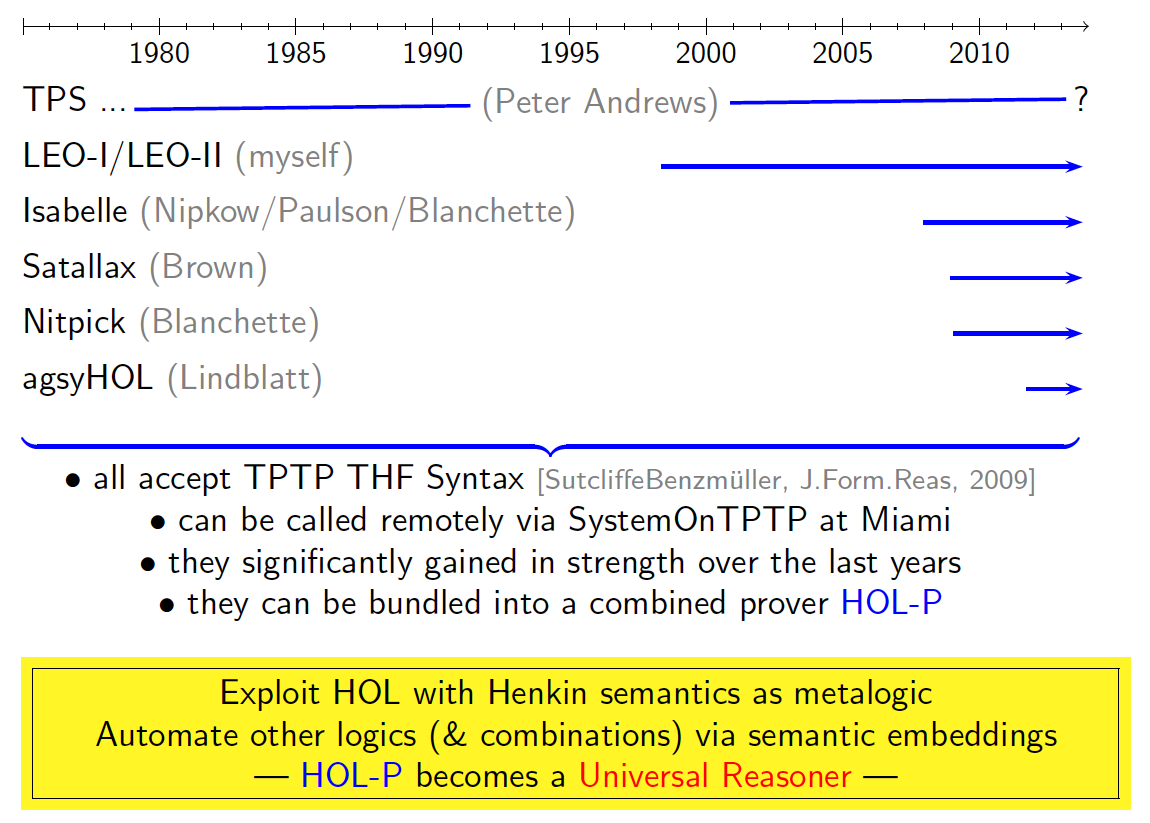
\includegraphics[width=1.05\textwidth]{$HOME/GoedelGod/Talks/FU-Berlin/Images/HOLProversGrab}
\end{frame}


% \begin{frame}{Proof Automation and Consistency Checking in THF and
%     TPI} \large
% \colorbox{gray}{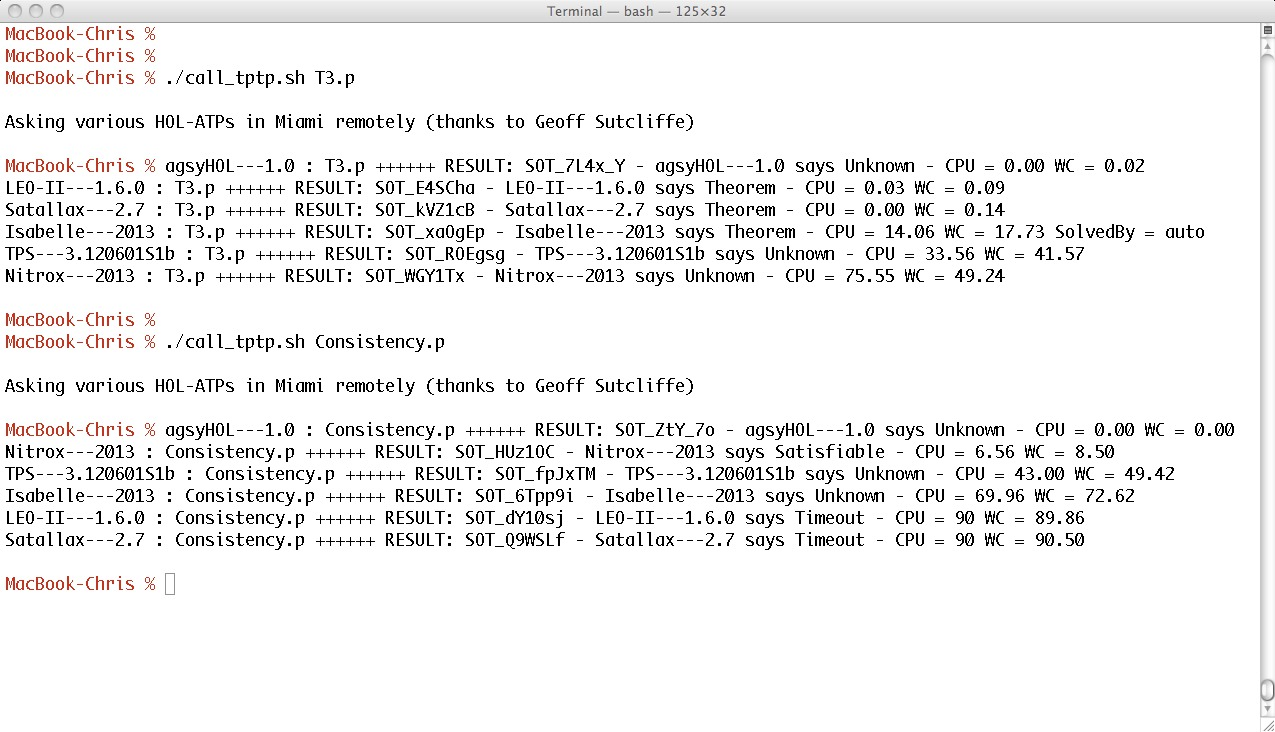
\includegraphics[width=\textwidth]{Images/Demos/DemoGrap}} 
% \vfill 
% {\scriptsize -- see THF files at:
%   \url{https://github.com/FormalTheology/GoedelGod/blob/master/Formalizations/THF/}
% --} 

% \medskip

% Provers are called remotely in Miami --- no local installation needed!
% \end{frame}


% \begin{frame}{The TPI Scripting Language}
% \begin{center}
%   \textcolor{red}{Cf. previous talk of Geoff Sutcliffe!}
% \end{center}
% \begin{itemize}
% \item Command and control instruction language for TPTP infrastructure
% \item Specify problems, avoiding repetitions
% \item Process the logical formulae: prove theorems, check
%   consistency, etc.
% \item Report results; exploit TPTP SZS ontology
% \item Fully automatic
% \item Very useful for reproducing experiments\\[1em]
% \end{itemize}

% Productive collaboration with Geoff: new features, debugging and testing
% \end{frame}

% \begin{frame}[t]{G�del's God as THF TPI Script}\tiny 
% \verbatiminput{verb1.txt}

% \onslide*<2->{
% \vskip-40em\hfill{\small \textcolor{red}{\Huge $\swarrow$}\colorbox{yellow}{\begin{minipage}[b]{7cm}\centering\phantom{.}\vskip.3em A (lean) QML prover in HOL \vskip.1em\phantom{.}\end{minipage}}}
% }
% \end{frame}

% \begin{frame}[t]{G�del's God as THF TPI Script}\tiny 
% \verbatiminput{verb2.txt}

% \onslide*<2>{
% \vskip-39em\hfill{\small \textcolor{red}{\Huge $\nwarrow$}\colorbox{yellow}{\begin{minipage}[t]{7cm}\centering\phantom{.}\vskip.3em Axiom B (symmetry) \vskip.1em\phantom{.}\end{minipage}}}
% }

% \onslide*<3>{
% \vskip-32em\hfill{\small \textcolor{red}{\Huge $\nwarrow$}\colorbox{yellow}{\begin{minipage}[t]{7cm}\centering\phantom{.}\vskip.3em Signature \vskip.1em\phantom{.}\end{minipage}}}
% }

% \onslide*<4>{
% \vskip-34em\hfill{\small \textcolor{red}{\Huge
%     $\swarrow$}\colorbox{yellow}{\begin{minipage}[b]{7cm}\centering\phantom{.}\vskip.3em
%       Definitions D1-D3 and Axiom A1(a/b) \vskip.1em\phantom{.}\end{minipage}}}
% }
% \end{frame}


% \begin{frame}[t]{G�del's God as THF TPI Script}\tiny
% \verbatiminput{verb3.txt}
% \onslide*<1>{
% \vskip-27em\hfill{\small \phantom{.}}
% }

% \onslide*<2>{
% \vskip-24em\hfill{\small \textcolor{red}{\Huge
%     $\nwarrow$}\colorbox{yellow}{\begin{minipage}[t]{7cm}\centering\phantom{.}\vskip.3em
%      Axioms A2-A5 \vskip.1em\phantom{.}\end{minipage}}}
% }

% \onslide*<3>{
% \vskip-22em\hfill{\small \textcolor{red}{\Huge
%     $\swarrow$}\colorbox{yellow}{\begin{minipage}[b]{7cm}\centering\phantom{.}\vskip.3em
%      Start checking consistency (asynchronously, Nitpick) \vskip.1em\phantom{.}\end{minipage}}}
% }

% \onslide*<4>{
% \vskip-15em\hfill{\small \textcolor{red}{\Huge
%     $\swarrow$}\colorbox{yellow}{\begin{minipage}[b]{7cm}\centering\phantom{.}\vskip.3em
%      Start checking consistency (asynchronously, LEO-II) \\ G�del's original definition of D2 \vskip.1em\phantom{.}\end{minipage}}}
% }
% \end{frame}

% \begin{frame}[shrink]{G�del's God as THF TPI Script}\tiny 
% \verbatiminput{verb4.txt}
% \onslide*<1>{
% \vskip-27em\hfill{\small \phantom{.}}
% }

% \onslide*<2>{
% \vskip-25em\hfill{\small \textcolor{red}{\Huge
%     $\nwarrow$}\colorbox{yellow}{\begin{minipage}[t]{7cm}\centering\phantom{.}\vskip.3em
%      Proving: T1 is a theorem (LEO-II)\vskip.1em\phantom{.}\end{minipage}}}
% }

% \onslide*<3>{
% \vskip-26em\hfill{\small \textcolor{red}{\Huge
%     $\swarrow$}\colorbox{yellow}{\begin{minipage}[b]{7cm}\centering\phantom{.}\vskip.3em
%      Proving: C is a theorem (LEO-II) \vskip.1em\phantom{.}\end{minipage}}}
% }
% \end{frame}

% \begin{frame}[shrink]{G�del's God as THF TPI Script}\tiny 
% \verbatiminput{verb5.txt}
% \onslide*<1>{
% \vskip-27em\hfill{\small \phantom{.}}
% }

% \onslide*<2>{
% \vskip-28em\hfill{\small \textcolor{red}{\Huge
%     $\nwarrow$}\colorbox{yellow}{\begin{minipage}[t]{7cm}\centering\phantom{.}\vskip.3em
%      Proving: T2 is a theorem  (LEO-II) \vskip.1em\phantom{.}\end{minipage}}}
% }

% \onslide*<3>{
% \vskip-30em\hfill{\small \textcolor{red}{\Huge
%     $\swarrow$}\colorbox{yellow}{\begin{minipage}[b]{7cm}\centering\phantom{.}\vskip.3em
%      Proving: T3 is a theorem  (LEO-II) \vskip.1em\phantom{.}\end{minipage}}}
% }
% \end{frame}

% \begin{frame}[shrink]{G�del's God as THF TPI Script}\tiny 
% \verbatiminput{verb6.txt}
% \onslide*<1>{
% \vskip-27em\hfill{\small \phantom{.}}
% }

% \onslide*<2>{
% \vskip-15em\hfill{\small \textcolor{red}{\Huge
%     $\nwarrow$}\colorbox{yellow}{\begin{minipage}[t]{7cm}\centering\phantom{.}\vskip.3em
%      Proving: C2 is a theorem  (LEO-II) \vskip.1em\phantom{.}\end{minipage}}}
% }

% \onslide*<3>{
% \vskip-18em\hfill{\small \textcolor{red}{\Huge
%     $\swarrow$}\colorbox{yellow}{\begin{minipage}[b]{7cm}\centering\phantom{.}\vskip.3em
%      Checking: Axioms are consistent (Nitpick)\vskip.1em\phantom{.}\end{minipage}}}
% }
% \end{frame}

% \begin{frame}[shrink]{G�del's God as THF TPI Script}\tiny 
% \verbatiminput{verb7.txt}
% \onslide*<1>{
% \vskip-27em\hfill{\small \phantom{.}}
% }

% \onslide*<2>{
% \vskip-23em\hfill{\small \textcolor{red}{\Huge
%     $\nwarrow$}\colorbox{yellow}{\begin{minipage}[t]{7cm}\centering\phantom{.}\vskip.3em
%      Checking: G�del's original axioms are inconsistent (LEO-II) \vskip.1em\phantom{.}\end{minipage}}}
% }

% \onslide*<3>{
% \vskip-26em\hfill{\small \textcolor{red}{\Huge
%     $\swarrow$}\colorbox{yellow}{\begin{minipage}[b]{7cm}\centering\phantom{.}\vskip.3em
%      Start checking modal collapse (asynchronously, LEO-II) \vskip.1em\phantom{.}\end{minipage}}}
% }

% \onslide*<4>{
% \vskip-15em\hfill{\small \textcolor{red}{\Huge
%     $\swarrow$}\colorbox{yellow}{\begin{minipage}[b]{7cm}\centering\phantom{.}\vskip.3em
%      Start checking 'flawlessness' of God (LEO-II)\vskip.1em\phantom{.}\end{minipage}}}
% }
% \end{frame}

% \begin{frame}[shrink]{G�del's God as THF TPI Script}\tiny 
% \verbatiminput{verb9.txt}
% \onslide*<1>{
% \vskip-27em\hfill{\small \phantom{.}}
% }

% \onslide*<2>{
% \vskip-18em\hfill{\small \textcolor{red}{\Huge
%     $\nwarrow$}\colorbox{yellow}{\begin{minipage}[t]{7cm}\centering\phantom{.}\vskip.3em
%      Checking: modal collapse holds (LEO-II)\vskip.1em\phantom{.}\end{minipage}}}
% }

% \onslide*<3>{
% \vskip-20em\hfill{\small \textcolor{red}{\Huge
%     $\swarrow$}\colorbox{yellow}{\begin{minipage}[b]{7cm}\centering\phantom{.}\vskip.3em
%      Checking: 'flawlessness' of God (LEO-II)\vskip.1em\phantom{.}\end{minipage}}}
% }
% \end{frame}


% \begin{frame}[shrink]{G�del's God as THF TPI Script}\tiny 
% \verbatiminput{verb10.txt}
% \onslide*<1>{
% \vskip-27em\hfill{\small \phantom{.}}
% }

% \onslide*<2>{
% \vskip-5em\hfill{\small \textcolor{red}{\Huge
%     $\nwarrow$}\colorbox{yellow}{\begin{minipage}[t]{7cm}\centering\phantom{.}\vskip.3em
%      Proving:Monotheism (TPS) \vskip.1em\phantom{.}\end{minipage}}}
% }

% \end{frame}


% \begin{transitionframe}{Images/Transitions/ReligiousSymbols(Sowlos)(CC-BY-SA).png}{white}
% \textbf{Part C:}

% Formalization and Verification in Coq
% \end{transitionframe}

% \begin{frame}{Coq Proof}{Demo}
% \begin{itemize}
% \item \begin{LARGE} Goal: verification of the natural deduction proof \end{LARGE}
% \begin{itemize}
% \item \begin{large} Step-by-step formalization \end{large}
% %\pause
% \item \begin{large} Almost no automation (intentionally!) \end{large}
% \end{itemize}
% %
% %\pause
% \item \begin{LARGE} Interesting facts: \end{LARGE}
% \begin{itemize}
% \item \begin{large} Embedding is transparent to the user \end{large}
% %\pause
% \item \begin{large} Embedding gives labeled calculus for free \end{large}
% \end{itemize}
% \end{itemize}
% \end{frame}

% \begin{frame}{Coq Proof}
% \colorbox{gray}{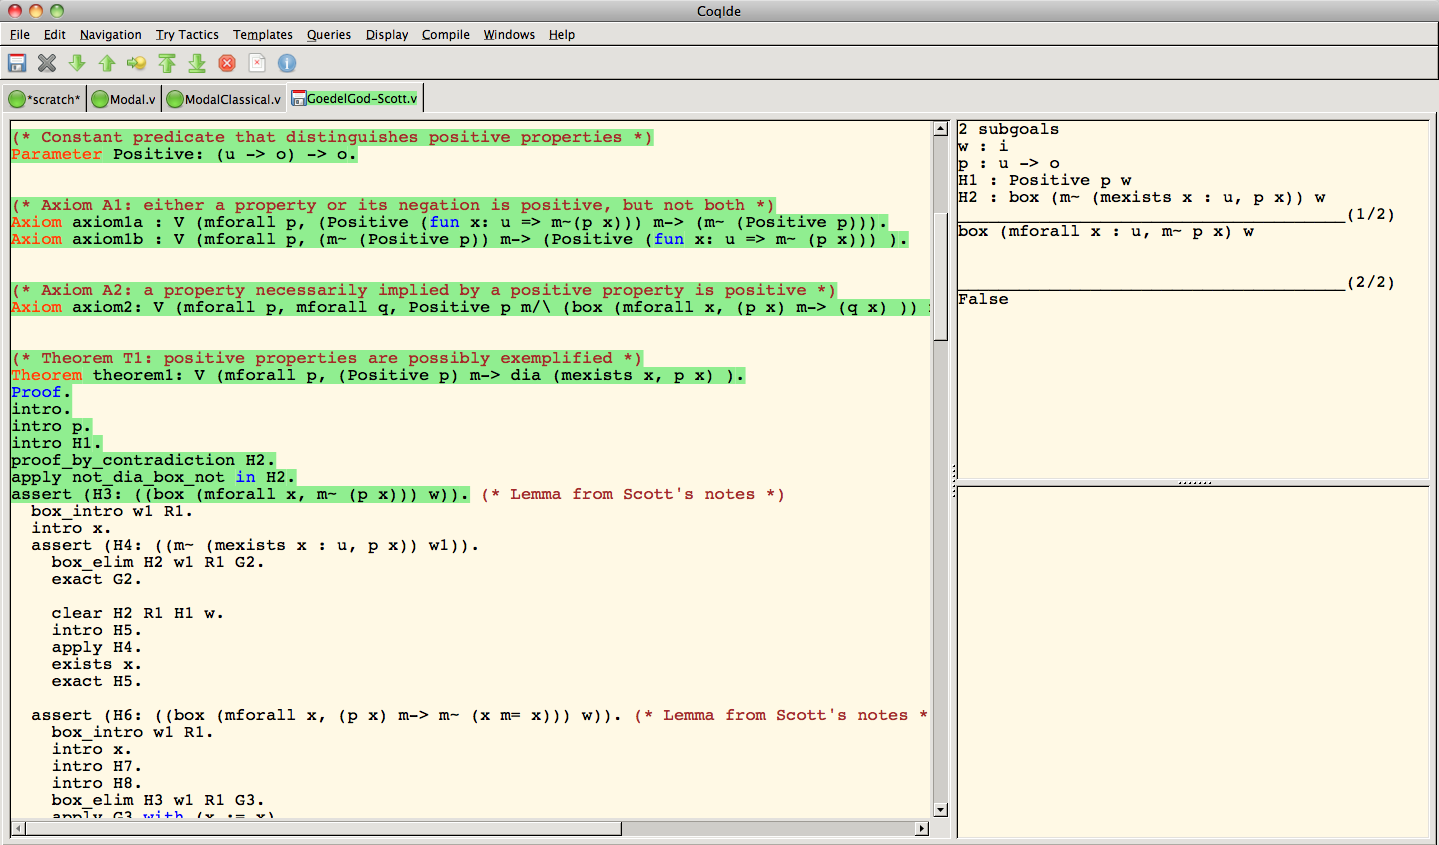
\includegraphics[width=\textwidth]{Images/Demos/CoqDemo.png}}
% \end{frame}



% \begin{transitionframe}{Images/Transitions/PaganReligions(CC-BY-SA).png}{white} \Large \centering
% \textbf{Part D:} \\[.5em]
% \quad Automation and Verification in \textsc{Isabelle/HOL} \\[2em]
% \end{transitionframe}

% \begin{frame}{} \Large \centering
% \vskip.5em
% \colorbox{gray}{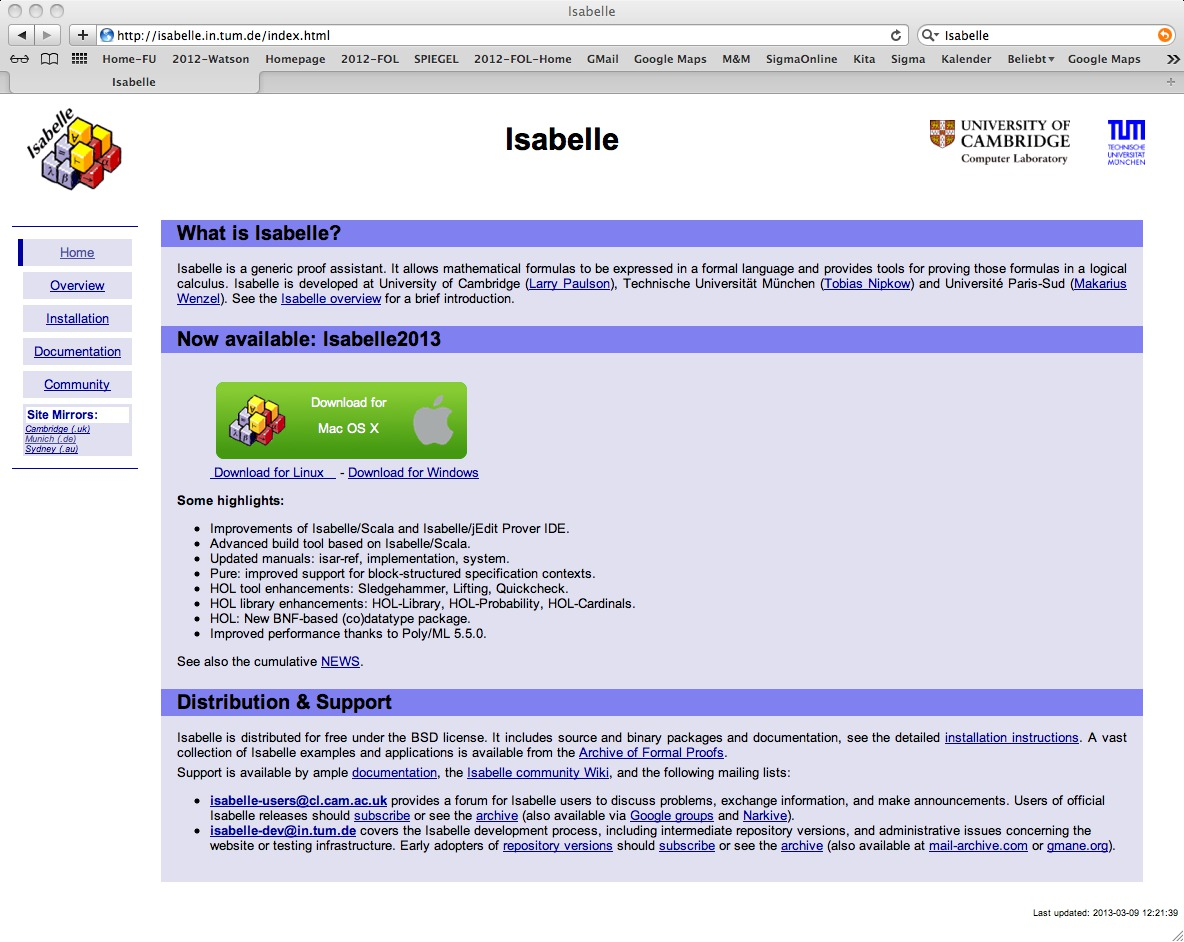
\includegraphics[width=\textwidth]{Images/IsabelleGrab}} 
% \end{frame}


% \begin{frame}{Automation \& Verification in Proof Assistant \textsc{Isabelle/HOL}} \large
% Isabelle/HOL   (Cambridge University/TU Munich)
% \begin{itemize}
% \item HOL instance of the generic \textsc{Isabelle} proof assistant
% \item User interaction and proof automation 
% \item Automation is supported by \textsc{Sledgehammer} tool
% \item Verification of the proofs in \textsc{Isabelle/HOL}'s small proof kernel
% \end{itemize}
% \vfill
% What we did?
% \begin{itemize}
% \item Proof automation of G\"odel's proof script (Scott's version)
% \item \textsc{Sledgehammer} makes calls to remote THF provers in Miami
% \item These calls the suggest respective calls to the \textsc{Metis} prover
% \item \textsc{Metis} proofs are verified in \textsc{Isabelle/HOL}'s proof kernel
% \end{itemize}
% \vfill
% \begin{center}
% --- see the handout (generated from the Isabelle source file) ---
% \end{center}
% \end{frame}


% \begin{frame}{Automation \& Verification in Proof Assistant
%     \textsc{Isabelle/HOL}} \large
% \colorbox{gray}{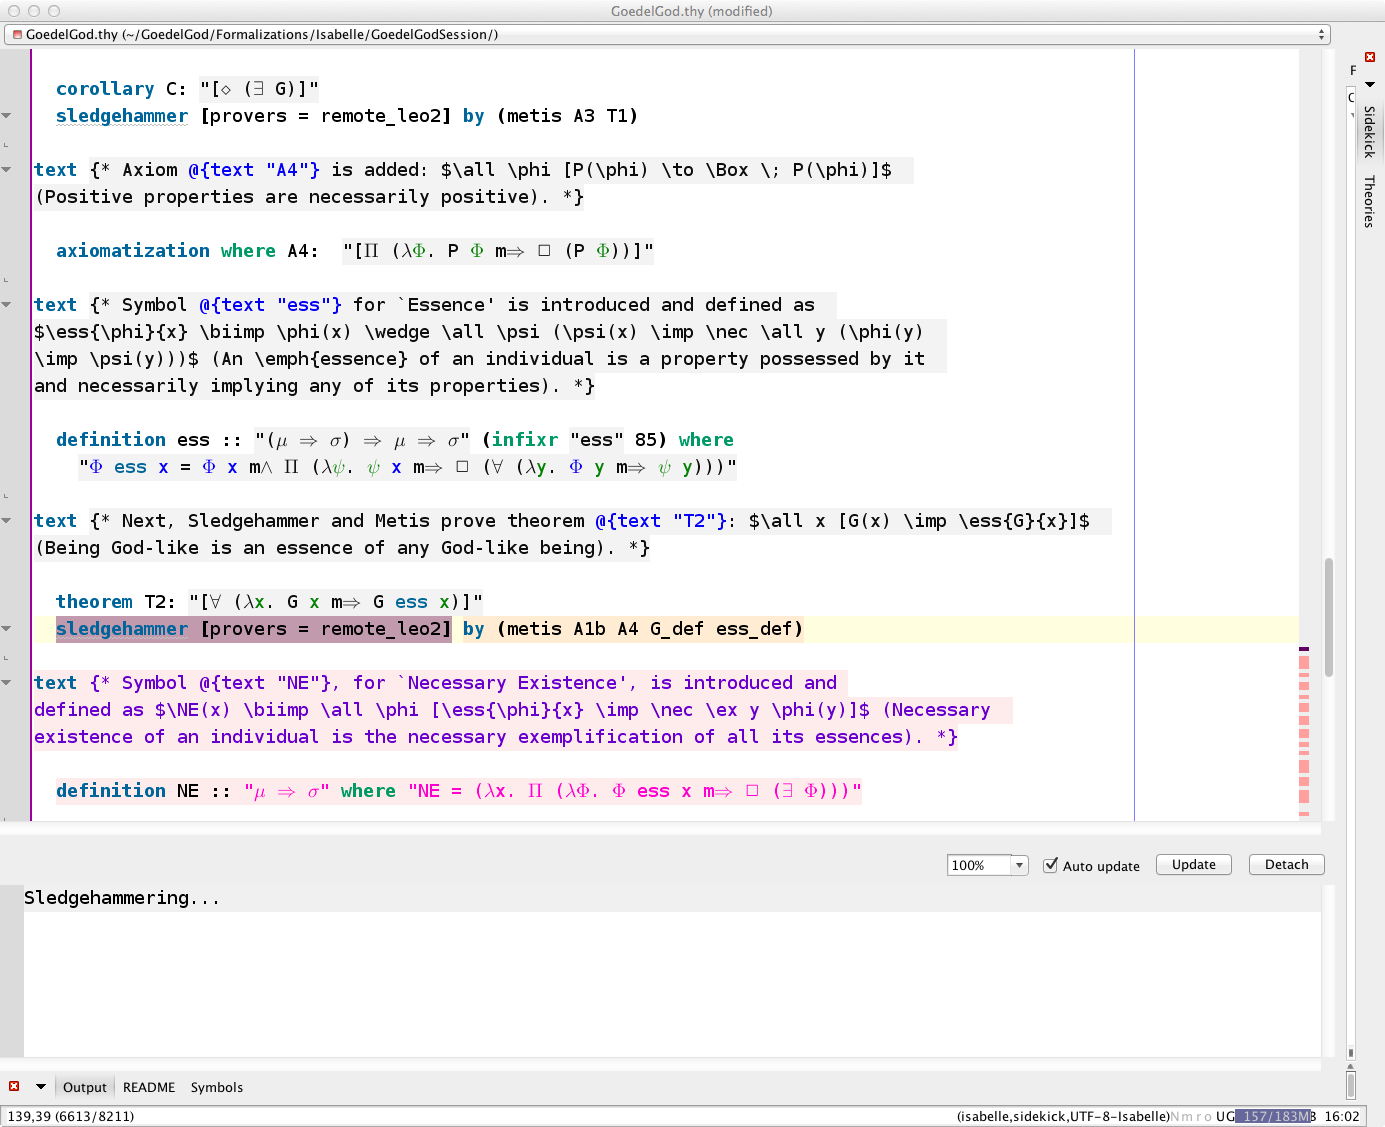
\includegraphics[width=.92\textwidth]{Images/Demos/IsabelleDemoGrab}} 
% \end{frame}




\begin{transitionframe}{$HOME/GoedelGod/Talks/FU-Berlin/Images/Transitions/NietzscheGod3}{black}
\textbf{Experiments and Results}
\end{transitionframe}


\begin{frame}{Scott's Version of G\"odel's Axioms, Definitions and
    Theorems}
\scottproof
\end{frame}


\begin{frame}{Proof Overview (in ND form)}
% G�del proves God's necessary existence by first 
% proving that, if God's existence is at all possible, 
% then it must be necessary (Lemma L). This idea is 
% already present in St. Anselm's and Descartes' 
% arguments. \\[1em]

% Leibniz argued that these arguments are 
% incomplete because they assumed the possibility of 
% God's existence (Corollary C) without any proof. 
% For Leibniz, this should be derivable from the 
% definition of God as a perfect being and from the 
% notion of perfection. This idea can be clearly 
% recognized in G�del's proof: from axioms A1 and A2, 
% one can derive that, for any positive property, 
% the existence of a being having this property is 
% possible (Theorem T1). \\[1em]

% As God is defined as a being 
% who possesses all positive properties, the property 
% of being God-like must be, by axiom A3, a positive 
% property as well.  C then follows trivially from T1.  \\[1em]

% The hardest lemmas in G�del's
% proof are T2 and L.  For that, G�del had to formulate a non-trivial
% definition of "essence", in order not only to derive T2 from A1 and A4
% but also to state an arguably acceptable axiom A5 allowing the
% derivation of L from T2 and other axioms from the modal logic S5.
\end{frame}

\begin{frame}{Experiments}\Large
\begin{itemize}
\item Formal encoding(s) of the axioms, definitions, and theorems in
  Scott's proof script
\item Calls to the HOL reasoners mentioned before
\item Interactive proofs in proof assistants Isabelle and Coq
\end{itemize}
\vfill
The source files of these experiments are available at:
\begin{center}
\url{https://github.com/FormalTheology/GoedelGod/}
\end{center}
\end{frame}

\begin{frame}[t]{Results} \Large
\begin{itemize}
\onslide*<1->{\item Axioms and definitions are consistent}
\onslide*<2->{\item Logic K is sufficient for proving T1, C and T2.}
\onslide*<2->{\item For proving the final theorem T3, logic KB is
  sufficient}

\onslide*<3>{\vfill\centering
\colorbox{yellow}{
\begin{minipage}{.9\textwidth}
Adresses criticisms: modal logic S5 is too strong
$$
\all P.[ \pos \nec P \imp \nec P ] 
$$
If something is possibly necessary, then it is necessary.
$$\pos\nec (A \vee \neg A)\qquad \nec(A \vee \neg A)$$
\alert{S5 usually considered adequate}

\textcolor{blue}{(But KB is sufficient! --- shown by HOL ATPs)}
\end{minipage}}}

\onslide*<4->{\item Only for T3 the HOL-ATPs still fail to produce a proof directly
  from the axioms; thus, T3 remains an interesting benchmark problem; T1, C, and T2 are rather trivial for HOL-ATPs.}
\onslide*<5->{\item G\"odel's original version of the proof.
  which omits conjunct $\phi(x)$ in the definition of \emph{essence}, 
  seems inconsistent.}
\end{itemize}
\end{frame}

\begin{frame}[t]{Results} \Large
\begin{itemize}
\onslide*<1->{\item G{\"o}del's axioms imply what is called the modal collapse
  $(\phi\supset\Box\phi)$, that is, contingent truth implies necessary
  truth.} 
\onslide*<2>{\vfill\centering
\colorbox{yellow}{
\begin{minipage}{.9\textwidth}
Fundamental criticism against G{\"o}del's argument. \\[1em]
Everything that is the case is so necessarily.\\[1em]
Follows from T2, T3 and D2 \textcolor{blue}{(as shown by HOL ATPs)}.\\[1em]
There are no contingent ``truths''. \\
Everything is determined. \\
There is no free will. \\[1em]
Many proposed solutions: Anderson, Fitting, H\'ajek, \ldots
\end{minipage}}}
\onslide*<3->{\item For proving T1, only the $\supset$-direction of A1 is
  needed. However, the $\subset$-direction of A1 is required for
  proving T2. Some philosophers try to avoid modal collapse by
  eluding/replacing the $\supset$-direction of A1.}
\onslide*<4->{\item G{\"o}del's axioms imply a `flawless god', that is, an entity
  that can only have `positive' properties.}
\onslide*<5->{\item Another implication of G{\"o}del's axioms is
  monotheism.} % MT can
  % easily be proved by Satallax from FG and D1. It remains non-trivial
  % to prove it directly from G{\"o}del's axioms.
\onslide*<6->{\item All of the above findings hold for both 

- constant domain semantics and 

- varying domain semantics (for the domain of individuals).}
\end{itemize}
\end{frame}

% \begin{frame}{Criticisms: Modal logic S5 is too strong} \centering \large
% $$
% \all P.[ \pos \nec P \imp \nec P ] 
% $$

% \medskip

% If something is possibly necessary, then it is necessary.

% \pause

% \bigskip


% $
% \pos\only<8->{_c} \nec\only<8->{_c} (A \vee \neg A)
% $
% \pause
% \qquad 
% $
% \nec\only<8->{_c} (A \vee \neg A)
% $

% \pause

% % \bigskip

% % logical necessity $\sim$ validity
% % %\qquad\qquad
% % \hfill
% % logical possibility $\sim$ satisfiability

% % \pause 

% % \medskip

% % $ 
% % \textrm{for all } M, M \models F 
% % \quad \longrightarrow \quad
% % \nec F
% % %\qquad\qquad\quad
% % \hfill
% % \textrm{exists } M, M \models F 
% % \quad \longrightarrow \quad
% % \pos F
% % $

% % \pause

% % \bigskip

% % \textbf{What about iterations?}
% % $$
% % \pos \nec \pos \pos F
% % $$

% % \medskip

% % \pause

% % weak intuitions $\Rightarrow$ dozens of modal logics

% \bigskip

% \pause

% \alert{S5 usually considered adequate}

% \medskip

% \pause

% \textcolor{blue}{(But KB is sufficient! --- shown by HOL ATPs)}


% \end{frame}


% \begin{frame}{Criticisms: G�del's Axioms imply Modal Collapse}
%   \centering \large
% $$
% \all P.[ P \imp \nec P ] 
% $$

% \medskip

% Everything that is the case is so necessarily.

% \pause

% \medskip

% Follows from T2, T3 and D2 \textcolor{blue}{(as shown by HOL ATPs)}.

% \pause

% \medskip

% There are no contingent ``truths''. \\ \pause
% Everything is determined. \\ \pause
% There is no free will. \\ \pause


% \pause
% \bigskip

% Many proposed solutions: Anderson, Fitting, H\'ajek, \ldots
 
% \end{frame}


% \begin{frame}{Criticisms: No Neutral Properties} \centering \large

% $$\all \phi [P(\neg \phi) \biimp \neg P(\phi)]$$

% Either a property is positive or its negation is (but never both)
		  
% \pause
% \bigskip

% Are the following properties positive or negative?

% $$
% \lambda x. G(x) \qquad \lambda x. NE(x) \qquad \lambda x. x = x  \qquad  \lambda x. \top
% $$
% \pause
% $$
% \lambda x. blue(x) \pause \qquad \lambda x. punishing(x) \pause \qquad \lambda x. human(x)
% $$

% %\pause

% %$$
% %\lambda x. foreigner(x) \qquad \lambda x. \neg foreigner(x), \ldots
% %$$

% \pause
% \medskip

% Solution: \\
% ``\ldots positive in the moral aesthetic sense (independently of the
% accidental structure of the world). Only then the ax. true. \ldots''
% \\ \hfill - G\"odel, 1970 

% \medskip

% See also my extended Isabelle formalization at: \url{https://github.com/FormalTheology/GoedelGod/blob/master/Formalizations/Isabelle/DivineVersion/GoedelGodDivine.thy}
% \end{frame}




\begin{transitionframe}{$HOME/GoedelGod/Talks/FU-Berlin/Images/Transitions/TrifidNebula(Nasa)(PublicDomain).jpg}{black}
\textbf{Conclusions}
\end{transitionframe}



% \begin{frame}{Summary of Results} \large

% The (\alert{new}) insights we gained from experiments include:\\[.5em]
% \begin{itemize}
% \item Logic K sufficient for T1, C and T2 
% \item Logic S5 not needed for T3
% \item \alert{Logic KB sufficient for T3 (not well known)}
% \item \alert{We found a simpler new proof of C}
% \item \alert{G\"odel's axioms (without conjunct $\phi(x)$ in D2) are inconsistent}
% \item Scott's axioms are consistent
% \item For T1, only half of A1 (A1a) is needed 
% \item For T2, the other half (A1b) is needed
% \end{itemize}
% \end{frame}


% \begin{frame}{Summary of Results} \large

% Our novel contributions to the theorem proving community include \\[.5em]
% \begin{itemize}
% \item Powerful infrastructure for reasoning with QML
% \item A new natural deduction calculus for higher-order modal logic
% \item Difficult new benchmarks problems for HOL provers
% \item Huge media attention
% \end{itemize}
% \end{frame}

\begin{frame}{Conclusion} \large
\vskip-1em What have we achieved \\[.5em]
\begin{itemize}
\item Verification of G\"odel's ontological argument with HOL provers
  \begin{itemize}
  \item exact parameters known: constant domain quantification, Henkin Semantics
  \item experiments with different parameters could be performed
  \end{itemize}
\item Gained some novel results and insights
\item Major  step towards \alert{Computer-assisted Theoretical Philosophy}
 \begin{itemize}
  \item see also Ed Zalta's \emph{Computational Metaphysics} project at Stanford University
  \item see also John Rushby's recent verification of Anselm's proof in PVS
  \item remember Leibniz' dictum --- \emph{Calculemus!}
  \end{itemize}
\item Interesting bridge between CS, Philosophy and Theology
\end{itemize}

\pause

\vfill
\vskip-1em Ongoing and future work \\[.5em]
\begin{itemize}
\item Formalize and verify literature on ontological arguments
  \begin{itemize}
  \item \ldots in particular the criticism and improvements to G\"odel 
  \end{itemize}
\item Own contributions --- supported by theorem provers
\end{itemize}
\end{frame}


% \begin{frame}{Some Comments and Reactions}
% \colorbox{gray}{
\includegraphics[width=.8\textwidth]{$HOME/GoedelGod/Talks/FU-Berlin/Images/Comments/Comment1}}\\[.7em]

% \, \hfill \colorbox{gray}{
\includegraphics[width=.7\textwidth]{Images/Comments/Comment2}}\\[.7em]

% \colorbox{gray}{
\includegraphics[width=.8\textwidth]{Images/Comments/Comment3}}\\[1em]

% \, \hfill \ldots find more on the internet \ldots
% \end{frame}

% \begin{frame}[plain]
% \colorbox{black}{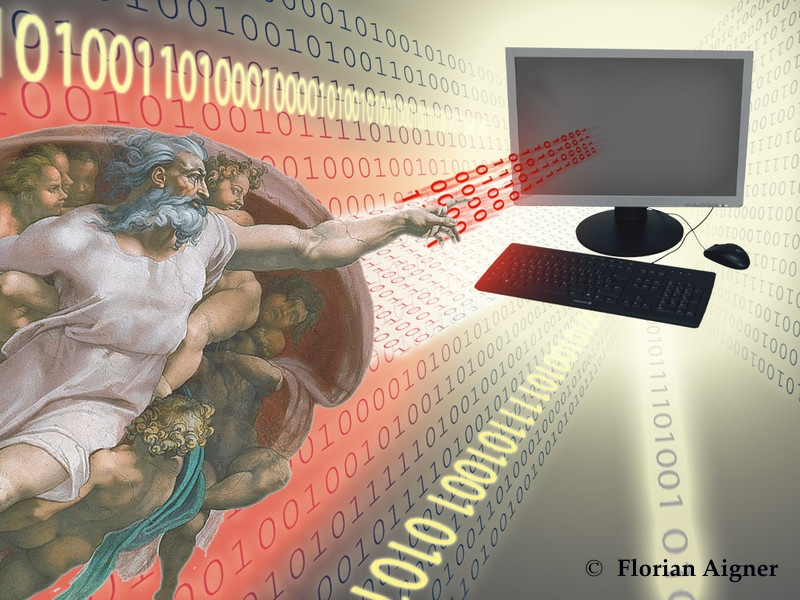
\includegraphics[width=\textwidth]{Images/Transitions/GodComputerC}}
% \end{frame}

% \begin{frame}{Licenses} \centering
% 
\includegraphics[scale=0.5]{Images/CC-BY-SA.png}

% \bigskip
% \bigskip

% \begin{center}
% The following images used in these slides were obtained in commons.wikimedia.org and are licensed as follows:

% \bigskip

% CC-BY-SA:

% ReligiousSymbols, PaganReligiousSymbols, NoGod.

% \bigskip

% Public Domain: 

% TrifidNebula
% \end{center}
% \end{frame}



\end{document}
